Per la pianificazione, sono stati individuati 4 fasi, scelte in base alle scadenze decise in comune accordo da tutto il gruppo. Ogni fase contiene diverse attività.\\

\noindent Dopo l'esperienza della fase 1, il gruppo ha pensato di ripianificare le successive fasi, rendendosi conto di aver valutato in maniera non efficiente la ripartizione di costi e risorse. In seguito alla decisione di ripianificare le attività, questa sezione è stata modificata in contenuto e struttura, fatta eccezione per la pianificazione della fase 1 il cui contenuto è rimasto invariato, in quanto già terminata. 
\subsection{Fase 1: Avvio e Analisi dei requisiti (2018-12-04 - 2019-01-21)}
		\subsubsection{Periodo di Avvio (2018-12-04 - 2018-12-17)}
		Nel periodo di avvio hanno luogo le seguenti attività:
		\begin{itemize}
			\item ricerca degli strumenti: tutti i membri del gruppo effettuano le ricerche sui possibili strumenti utili alle attività di avvio e di analisi dei requisiti;
			\item prima normazione: gli amministratori redigono le \textit{NormeDiProgetto\_v2.0.0} concordate per i processi di supporto e organizzativi;
			\item studio di fattibilità: gli analisti redigono lo \textit{StudioDiFattibilità\_v2.0.0} dei capitolati;
			\item pianificazione di progetto: il responsabile redige il \textit{PianoDiProgetto\_v2.0.0}, riportando modello di sviluppo, analisi dei rischi e la pianificazione per le prime attività dell'analisi dei requisiti;
			\item verifica dei documenti: i verificatori controllano che i documenti siano corretti.
		\end{itemize}
		
	\subsubsection{Periodo di Analisi dei Requisiti (2018-12-18 - 2019-01-21)}	
 Il periodo di analisi dei requisiti inizia con le attività di:
			\begin{itemize}
				\item pianificazione di progetto: il responsabile effettua il resoconto del periodo di avvio e pianifica in maniera più dettagliata le attività di analisi dei requisiti; 
				\item pianificazione della qualifica: i verificatori redigono il resoconto del periodo di avvio e gli amministratori effettuano i primi incrementi per il \textit{PianoDiQualifica\_v2.0.0};
				\item normazione: gli amministratori redigono in maniera precisa e completa le \textit{Norme di progetto} per l'attività di analisi;
				\item verifica dei documenti: si procede con la verifica del \textit{PianoDiProgetto\_v2.0.0}, del \textit{PianoDiQualifica\_v2.0.0} e delle \textit{NormeDiProgetto\_v2.0.0}.
				\item analisi dei requisiti del sistema: gli analisti svolgono la prima analisi dei requisiti del sistema;
				\item incrementi al \textit{PianoDiQualifica\_v2.0.0}: i verificatori introducono nel piano i test di sistema in base a quanto scaturito dall'analisi dei requisiti;
				\item verifica dell'analisi dei requisiti di sistema;
				\item incrementi all'analisi dei requisiti: gli analisti aggiungono degli incrementi all'analisi di sistema;
				\item verifica degli incrementi all'analisi dei requisiti;
				\item incrementi al \textit{PianoDiProgetto\_v2.0.0}: il responsabile redige la parte di rendicontazione e consuntivo del \textit{PianoDiProgetto\_v2.0.0} da presentare alla Revisione dei Requisiti.
				\item incrementi al \textit{Piano di qualifica}: i verificatori redigono la parte di rendicontazione del \textit{PianoDiQualifica\_v2.0.0} da presentare alla Revisione dei Requisiti, aggiungendo i risultati delle misurazioni effettuate, e gli analisti aggiungono i restanti test di sistema;
				\item verifica del \textit{PianoDiProgetto\_v2.0.0} e del \textit{PianoDiQualifica\_v2.0.0};
				\item approvazione dei documenti da parte del responsabile;
				\item preparazione alla presentazione.			
			\end{itemize}
			
\begin{figure}[h]
	\centering
	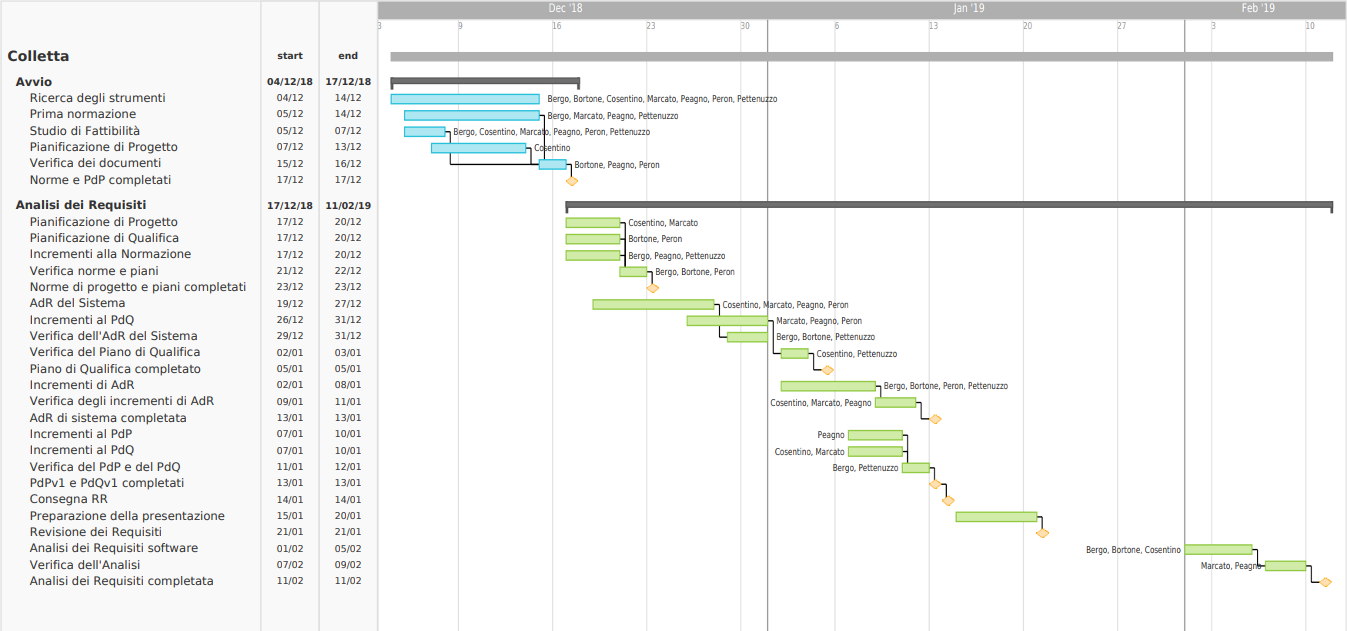
\includegraphics[scale=0.33]{images/ganttan.png}
	\caption{Diagramma di Gantt riguardante la fase 1}
\end{figure}

\subsection{Fase 2: Progettazione della base tecnologica (2019-01-22 - 2019-03-15)}	
	Nella fase 2 si svolgeranno le seguenti attività:
\begin{itemize}
	\item normazione: modifiche alle \textit{Norme di progetto} secondo quanto segnalato alla Revisione dei requisiti. Si procede poi con il suo incremento;
	\item pianificazione della qualifica: modifiche al \textit{Piano di qualifica} secondo quanto segnalato alla Revisione dei requisiti. Si procede poi con il suo incremento;
	\item pianificazione delle attività: modifiche al \textit{Piano di progetto} secondo quanto segnalato alla Revisione dei requisiti;
	\item analisi dei requisiti: modifiche al \textit{Analisi dei requisiti} secondo quanto segnalato alla Revisione dei requisiti;
	\item progettazione PoC e Technology Baseline: vengono ricercate le tecnologie, i framework e le librerie ritenute più adatte allo sviluppo del prodotto;
	\item codifica: realizzazione del PoC;
	\item verifica per il colloquio: verifica del PoC in vista di una discussione Agile con il committente;
	\item colloquio: viene effettuato il colloquio con la committente;
	\item incremento progettazione e codifica: in base alla segnalazioni ricevute durante il colloquio con il committente vengono eseguite opportune modifiche;
	\item incremento della pianificazione delle attività: viene aggiornato il \textit{Piano di progetto} con il consuntivo riguardante la fase 2;
	\item verifica per la consegna: vengono verificati tutti i documenti e la Technology Baseline con la relativa codifica;
	\item consegna del materiale in ingresso;
	\item preparazione alla presentazione.
\end{itemize}

\begin{figure}[h]
	\centering
	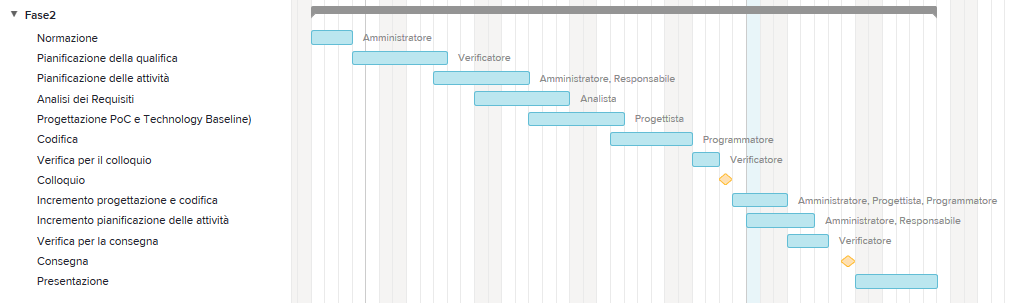
\includegraphics[scale=0.67]{images/fase2.png}
	\caption{Diagramma di Gantt riguardante la fase 2}
\end{figure}
	
\subsection{Fase 3: Progettazione di dettaglio e codifica (2019-03-16 - 2019-04-19)}
	Nella fase 3 hanno luogo le seguenti attività:
\begin{itemize}
	\item normazione: modifiche alle \textit{NormeDiProgetto\_v2.0.0} secondo quanto segnalato alla Revisione di progettazione. Si procede poi con il suo incremento;
	\item pianificazione della qualifica: modifiche al \textit{PianoDiQualifica\_v2.0.0} secondo quanto segnalato alla Revisione di Progettazione. Si procede poi con il suo incremento;
	\item pianificazione delle attività: modifiche al \textit{PianoDiProgetto\_v2.0.0} secondo quanto segnalato alla Revisione di progettazione;
	\item progettazione in dettaglio e Product Baseline: questa attività consiste nella progettazione del prodotto tramite diagrammi delle classi e di sequenza, incrementando quanto sviluppato nel PoC.
	\item codifica: realizzazione del prodotto;
	\item verifica per il colloquio: verifica del codice scritto in vista del colloquio Agile con il committente;
	\item colloquio: viene effettuato il colloquio con il committente;
	\item redazione manuali: redazione \textit{Manuale Utente} e \textit{Manuale Sviluppatore};
	\item incremento progettazione e codifica: in base alle segnalazioni ricevute al colloquio con il committente viene eseguito l'eventuale incremento;
	\item incremento della pianificazione delle attività: viene aggiornato il \textit{Piano di Progetto} con il consuntivo pre-finale;
	\item verifica per la consegna: vengono verificati tutti i documenti e il Product Baseline con la relativa codifica;
	\item approvazione dei documenti da parte del responsabile. Sono pronti per il rilascio le \textit{NormeDiProgetto\_v3.0.0}, il \textit{PianoDiProgetto\_v3.0.0}, il \textit{PianoDiQualifica\_v3.0.0}, l'\textit{AnalisiDeiRequisiti\_v3.0.0}, il
	\textit{ManualeUtente\_v1.0.0} e il \textit{ManualeSviluppatore\_v1.0.0}
	\item preparazione alla presentazione.
\end{itemize}

\begin{figure}[h]
	\centering
	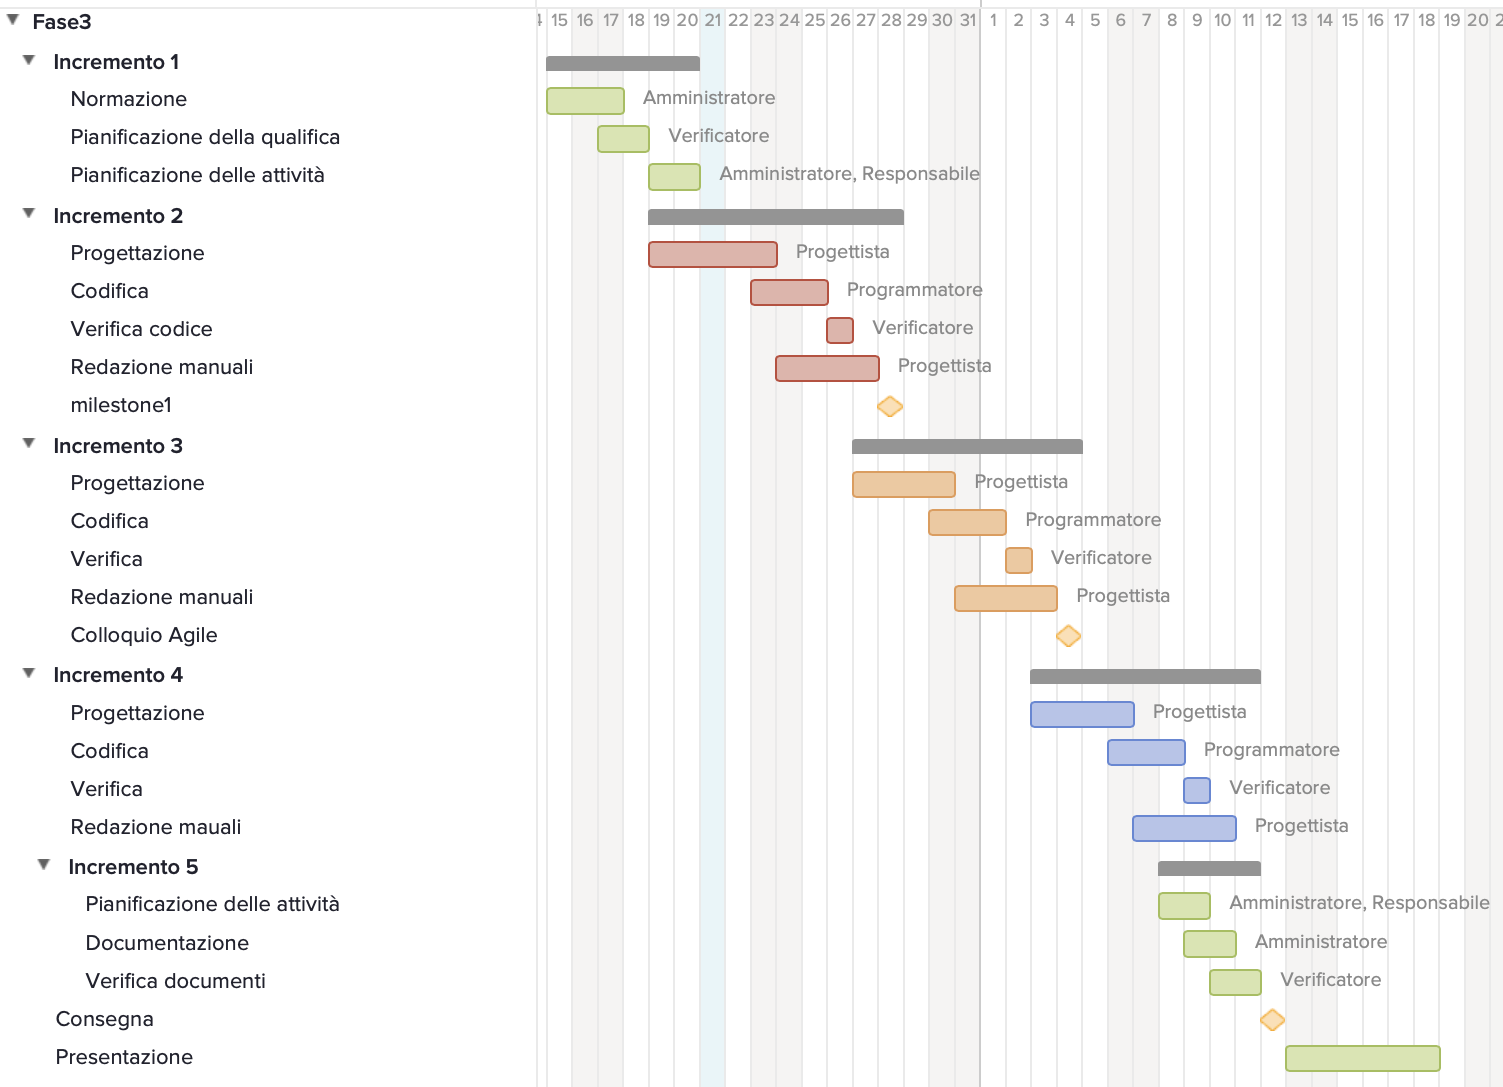
\includegraphics[scale=0.70]{images/fase3.png}
	\caption{Diagramma di Gantt riguardante la fase 3}
\end{figure}
	
\subsection{Fase 4: Validazione e collaudo (2019-04-21 - 2019-05-17)}
	Nella fase 4 vengono eseguite le seguenti attività:
\begin{itemize}
	\item normazione: modifiche alle \textit{Norme di progetto} secondo quanto segnalato alla Revisione dei requisiti. Si procede poi con il suo incremento;
	\item pianificazione della qualifica: modifiche al \textit{PianoDiQualifica\_v2.0.0} secondo quanto segnalato alla Revisione di qualifica; Si procede poi con il suo incremento;
	\item pianificazione delle attività: modifiche al \textit{PianoDiProgetto\_v2.0.0} secondo quanto segnalato alla Revisione di qualifica;
	\item progettazione di dettaglio: incremento al \textit{Product Baseline} con secondo quanto segnalato alla Recisione di qualifica;
	\item codifica: codifica degli incrementi effettuati durante la progettazione;
	\item redazione manuali: incrementi al \textit{ManualeUtente\_v2.0.0} e al \textit{ManualeSviluppatore\_v2.0.0} in base a quanto segnalato alla Revisione di qualifica;
	\item verifica: verifica degli incrementi effettuati;
	\item validazione e collaudo: vengono eseguiti i test di qualifica e il collaudo per il rilascio;
	\item preparazione alla presentazione;
	\item consegna del materiale in ingresso.
\end{itemize}

\begin{figure}[h]
	\centering
	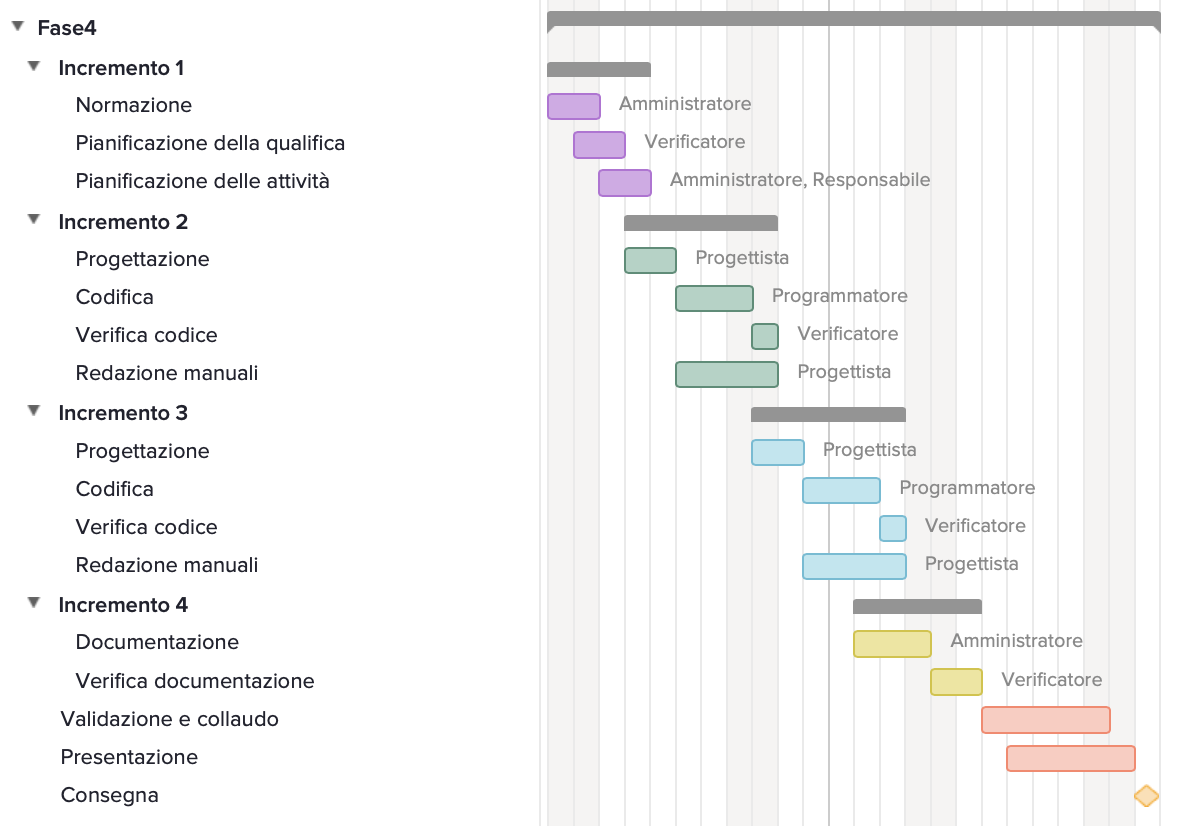
\includegraphics[scale=0.70]{images/fase4.png}
	\caption{Diagramma di Gantt riguardante la fase 4}
\end{figure}
	
\newpage